\section{Discussion}
\label{sec:discussion}

This research has explored how regular expressions are used in practice. In this section, we discuss the implications of these empirical findings on tool designers and users of regex tools and opportunities for future work.



\subsection{Implications For Tool Designers of Omitting a Feature}

We observe that, although the clusters were generated based on behavioral similarity, they are often centered around the presence of certain features. Thus, omitting those features in a tool's implementation often omits an entire space of regular expression behaviors.


\subsubsection{STR, END}
The endpoint anchor features STR and END are the only way to specify that the entire input string has to match a pattern.  Consider the following example, comparing the pattern \verb!`^\s*$'! to the pattern \verb!`\s*'! when looking for input strings devoid of content.  Because it does not have endpoint anchors, the pattern \verb!`\s*'! matches all inputs, since there are always at least zero whitespace characters in every input.  But with the endpoint anchors, only inputs that contain nothing but whitespace will match, allowing the user to determine if a string is devoid of content.

From Table~\ref{table:featureStats} we know that STR and END features are present in over half of the scanned projects containing utilizations - further evidence of the importance of these features.  The brics library does not support this feature, which is a missed opportunity for many developers who could otherwise have used brics to model their regexes that use STR and END.

\subsubsection{LZY}
The LZY feature modifies the behavior of the repetition features (i.e., ADD, KLE, QST, DBB, LWB, SNG) by forcing them to use as few repetitions as possible for a match.  The default behavior for the repetition features is to use as many repetitions as possible for a match.  Consider trying to find the shortest sequence of binary characters starting and ending with a 1 within the binary sequence: {\tt 1010001}. The pattern \verb!`1.*1'! will match the entire sequence whereas the pattern \verb!`1.*?1'! will match {\tt 101} because the KLE repetition feature was modified by the LZY feature.  There is no way to obtain shortest matches without the LZY feature.  LZY is present in over 36\% of scanned projects with utilizations (see Table~\ref{table:featureStats}), and yet was not supported by two of the four major regex projects we looked at.

\subsection{Key User Behaviors to Support}
%Several key user behaviors were observed in the corpus of patterns, and in the clusters and cluster categories that...
Here we offer a discussion of the main behaviors that are important for tool designers to support.

\subsubsection{Prioritized List of Features}
\label{sec:prioritizedList}
Based on our analysis of feature usage in RQ2 and the data presented in Table~\ref{table:featureStats}, we have produced a prioritized list of features (Figure~\ref{fig:prioritizedList}) to include in a tool meant to support as many regexes as possible.

\begin{figure}[tb]
\fbox{\parbox{\columnwidth}{
\begin{enumerate}
\item literals, sequences of tokens
\item CCC (NCCC, RNG, WSP, DEC, WRD, NWSP, NDEC, NWRD)
\item CG (without back-references)
\item DBB (ADD, KLE, QST, SNG, LWB)
\item STR, END
\item OR
\item LZY
\item NCG
\item NLKA, LKA, NLKB, LKB
\item WNW, NWNW
\item ENDZ
\item BKR
\end{enumerate}
}}
\caption{A Suggested Feature Implementation Priority List \label{fig:prioritizedList}
}
\end{figure}

The features NCCC, RNG, WSP, DEC, WRD, NWSP, NDEC, NWRD are all included as the second priority because by implementing CCC, these features are available as specific instances of CCC.  Consider how the DEC feature can be simulated using CCC, for example  $\backslash d \equiv [0123456789]$. Likewise, any use of the RNG feature can be simulated using CCC, for example: $[a-f] \equiv [abcdef]$.

Similarly, the features ADD, KLE, QST, SNG and LWB are available once the DBB feature is implemented.  Consider how every use of the ADD feature can be simulated with a specific use of the DBB feature, for example: $a+ \equiv a\{1, MAX\}$.  In the same way, any use of the SNG feature can be simulated using the DBB feature, for example:  $a\{5\} \equiv a\{5, 5\}$.


\subsubsection{Capturing Specific Content}
As mentioned in section~\ref{sec:featureUsage}, the CG feature is the most frequently used feature in terms of patterns and files (see Table~\ref{table:featureStats}).  The ability to capture some part of a match provides a powerful tool to programmers.  As mentioned in Section~\ref{sec:clusterResults}, capturing values assigned to variables was one of the main categories of clusters observed.  All four of the major regex tools support the CG feature.  Any non-trivial tool or research that hopes to be applicable to regex use in practice must treat the CG feature as especially important.

\subsubsection{Use of the Default Character Classes}
The pattern language for Python and most major regex engines support a few default character classes (and their negations) which we have described as the features ANY, DEC, WSP, WRD, NDEC, NWSP, NWRD.  Throughout this analysis it was obvious that these default character classes were widely used.  As mentioned in section~\ref{sec:prioritizedList}, all of these default character classes can be simulated using the CCC feature, and the CCC feature is one of the most basic features that is essential for all regex tools to support.  For tools that do not support the default character classes, this is a significant obstacle for users trying to test or model the regexes that they already have.

\subsubsection{Using {\tt`.*'} to Count Lines Containing a Pattern}
Text files containing one unit of information per line are common in a wide variety of applications (for example log and csv files).  Out of all the patterns observed during this study, the most ubiquitous sub-pattern was \verb!`.*'!, usually present near the end of the pattern.  Out of the 13,912 patterns in the corpus, 3444 (24\%) contained \verb!`.*'! at least once.
One reasonable explanation for this tendency to put \verb!`.*'! at the end of a pattern is that users want to disregard all matches after the first match on a single line in order to count how many distinct lines the match occurs on, as illustrated in Figure~\ref{fig:lineSearch}.  Tools that intend to be applicable to regex use in practice must support both the ANY and KLE features, and should give special care to maintain the expected line-counting behavior for the \verb!`.*'! idiom.

%\subsubsection{Using `\textbackslash W' to Sanitize Arbitrary Text}


\begin{figure}[tb]
\centering
\fbox{
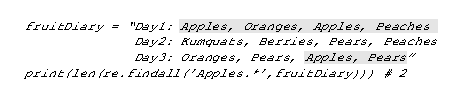
\includegraphics[width=\columnwidth]{../illustrations/lineSearch.eps}
}
\caption{An Example of Using .* to Count Lines Containing `Apples' \todo{crop}}
\label{fig:lineSearch}
\end{figure}


\subsection{Opportunities For Future Work}

Based on our findings, there are many opportunities for future work.

\subsubsection{Re-Evaluating the WRD Character Class}
One surprising result of our clustering is that, behaviorally speaking, the negation of the word class NWRD was used in 208 projects, while the word class itself was used in only 114 projects. After inspecting several projects using the patterns found in this behavioral cluster, we concluded that most users are trying to sanitize arbitrary strings that must conform to a system character set requirement, such as requirements for filenames.  For example, a user might replace all NWRD matching characters with the `\_' to guarantee that an arbitrary string can be used as a filename.  We also considered the largest cluster using custom character classes (\verb•[^ -~](122)•) and concluded that users are constructing a more permissive version of the NWRD character class, to allow more non-letter, non-digit characters than just the `\_' in their sanitized strings.  We hypothesize that this is because modern systems allow more special characters in filenames than systems allowed when the WRD character class originated.  More research is needed to determine if a more modern WRD class could be useful, and if so, what characters set is preferred.

% \subsubsection{How Does Developer Experience Influence Regex Composition?}
% % \noindent \emph{Observation 1: Utilizations May Be More Common In Python Library Code Than In User Code. }
% The project with the most files containing utilizations observed is Arianrhod\footnote{\url{https://github.com/Ouroboros/Arianrhod}} which is a Japanese Anime game, mostly written in C\# (over 18K files), but containing 3404 Python files.  Most of these Python files are source code for various libraries.  Of these library files, 15.9\% (541) contain at least one utilization, which is more than the 11\% average.  This indicates that more experienced developers (those capable of developing core Python libraries) may be more likely to use regexes than less experienced developers.  More research is needed to determine if experienced developers are more likely to use regexes, and what differences in feature set and composition can be observed when compared to regexes composed by less experienced developers.

\subsubsection{Regexes need refactoring}
When clustering by behavior, we observed many clusters with more than 10 patterns all specifying nearly the same behavior.  We don't know why different users choose to implement the same behavior in different ways.  Out of the 13,912 patterns in the corpus, 1977 (14\%) used the RNG feature to specify the range \verb•0-9•, even though this is exactly equivalent to using \verb•\d• .  Future work is needed to determine why users specify digits using the RNG feature when an equivalent default character class already exists, as has been done for other refactoring work (e.g.,~\cite{StoleeTSE2013}). 

% \subsubsection{dot-star at the end - refactoring?}
% One of the most ubiquitous sub-patterns, \verb!`.*'! appeared in 1937 of the 9727 patterns acceptable by Rex, and appeared within the last four characters in 1161 of the 9727 patterns.  Out of the top 30 clusters containing the ANY feature, 26 also had \verb!`.*'! within the last four characters.






% In many cases, this \verb!`.*'! at the end of the string may not actually contribute any new behavior to the pattern, and may in fact be extraneous.  Or users may be trying to bypass the whole-string nature of the {\tt re.match} function, without realizing that they could instead use the {\tt re.search} function.  Consider the comparison shown in Figure~\ref{fig:searchVSmatch}

% \begin{figure}[tb]
% \centering
% \fbox{
% 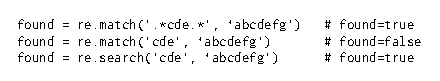
\includegraphics[width=\columnwidth]{../illustrations/matchVSsearch.eps}
% }
% \caption{An Example of Using .* to get Search Behavior From The Match Function}
% \label{fig:searchVSmatch}
% \end{figure}

% Are programmers using the dot-star sub-pattern unnecessarily? More research is needed into this question to find out if these patterns are a candidate for refactoring.



% to find the largest count for the 'utilizing files' row: select distinct uniqueSourceID, filePath, count(distinct filePath) as ct from RegexCitationMerged group by uniqueSourceID order by ct;


% \subsubsection{default character classes are widely used}

%  Specifically, \verb!\s!, \verb!\d! and \verb!\W! were the top three behavioral clusters (as shown in Table~\ref{table:topNClusters}).  In Table~\ref{table:threeClusterSample} we show the top 10 patterns from these top three clusters. \todo{implication for tool designers}

% 
\begin{table}
\begin{center}
\caption{Top 10 Patterns in Top 3 Clusters (RQ3)}
\label{table:threeClusterSample}

\begin{tabular}
{c|c|c}
\toprule
example & example & example\\
\midrule
\begin{minipage}{0.5in}\begin{verbatim}`\s'\end{verbatim}\end{minipage} & \begin{minipage}{0.5in}\begin{verbatim}`\s'\end{verbatim}\end{minipage} & \begin{minipage}{0.5in}\begin{verbatim}`\s'\end{verbatim}\end{minipage}\\
\midrule
\begin{minipage}{0.5in}\begin{verbatim}`\s'\end{verbatim}\end{minipage} & \begin{minipage}{0.5in}\begin{verbatim}`\s'\end{verbatim}\end{minipage} & \begin{minipage}{0.5in}\begin{verbatim}`\s'\end{verbatim}\end{minipage}\\
\midrule
\begin{minipage}{0.5in}\begin{verbatim}`\s'\end{verbatim}\end{minipage} & \begin{minipage}{0.5in}\begin{verbatim}`\s'\end{verbatim}\end{minipage} & \begin{minipage}{0.5in}\begin{verbatim}`\s'\end{verbatim}\end{minipage}\\
\midrule
\begin{minipage}{0.5in}\begin{verbatim}`\s'\end{verbatim}\end{minipage} & \begin{minipage}{0.5in}\begin{verbatim}`\s'\end{verbatim}\end{minipage} & \begin{minipage}{0.5in}\begin{verbatim}`\s'\end{verbatim}\end{minipage}\\
\midrule
\begin{minipage}{0.5in}\begin{verbatim}`\s'\end{verbatim}\end{minipage} & \begin{minipage}{0.5in}\begin{verbatim}`\s'\end{verbatim}\end{minipage} & \begin{minipage}{0.5in}\begin{verbatim}`\s'\end{verbatim}\end{minipage}\\
\midrule
\begin{minipage}{0.5in}\begin{verbatim}`\s'\end{verbatim}\end{minipage} & \begin{minipage}{0.5in}\begin{verbatim}`\s'\end{verbatim}\end{minipage} & \begin{minipage}{0.5in}\begin{verbatim}`\s'\end{verbatim}\end{minipage}\\
\midrule
\begin{minipage}{0.5in}\begin{verbatim}`\s'\end{verbatim}\end{minipage} & \begin{minipage}{0.5in}\begin{verbatim}`\s'\end{verbatim}\end{minipage} & \begin{minipage}{0.5in}\begin{verbatim}`\s'\end{verbatim}\end{minipage}\\
\midrule
\begin{minipage}{0.5in}\begin{verbatim}`\s'\end{verbatim}\end{minipage} & \begin{minipage}{0.5in}\begin{verbatim}`\s'\end{verbatim}\end{minipage} & \begin{minipage}{0.5in}\begin{verbatim}`\s'\end{verbatim}\end{minipage}\\
\midrule
\begin{minipage}{0.5in}\begin{verbatim}`\s'\end{verbatim}\end{minipage} & \begin{minipage}{0.5in}\begin{verbatim}`\s'\end{verbatim}\end{minipage} & \begin{minipage}{0.5in}\begin{verbatim}`\s'\end{verbatim}\end{minipage}\\
\midrule
\begin{minipage}{0.5in}\begin{verbatim}`\s'\end{verbatim}\end{minipage} & \begin{minipage}{0.5in}\begin{verbatim}`\s'\end{verbatim}\end{minipage} & \begin{minipage}{0.5in}\begin{verbatim}`\s'\end{verbatim}\end{minipage}\\
\bottomrule
\end{tabular}
\end{center}
\end{table}



% example with anchors and {\tt .*} in the middle which could be replaced by a comma?














% Fun fact: while creating similarity matrix, row 5464 took 2 hours, or almost 1 second per cell avg, only suffering 18 timeouts (1.2 secs).  What is this pesky pattern?

% We do not assume that Python projects represent a perfect sample of regular expression usage in all environments, but to make the work of collecting data for the paper reasonable, we had to choose one language to focus on (we hope to compare results across languages in future work).  Python is an attractive choice because the culture of Python programming makes it seem likely that someone would write the pattern directly in the function, not trying to over-complicate things with some extra Classes or functions.  Other attractive choices are Perl (which probably has the most active regex community), javascript and ruby (which may emphasize web tasks like form validation), sql or a general purpose language like java or C\#.


% \todo{What does it mean when WSP is more pervasive in patterns and files, but not projects.  That it is popular among those who are used to using it but not everyone is used to using it? Stronger correlation between nPatterns and nFiles vs nFiles and nProjects or nPatterns and nProjects}

% \todo{NDEC is one of the most rarely used features, while DEC is one of the most frequently used default char classes.  Contrast this with the craving for NWRD behavior evident from clustering.}

% \subsubsection{An Evaluation of the Functions and Flags}

% ACKk somesection about flags: notice how rarely the LOCALE flag was used, how combined flags were never used, and certain functions were almost never used.

%Notice that the presence of the Verbose flag implies usage of the comment feature!



